\chapter{Experiments/Evaluation}
\label{sec:evaluation}
%Why we need evaluation\label{sec:relevance}

The main contribution of this paper is to introduce a new approach for explanations(Hierarchical Intervention). We evaluate this new approach in a number of different ways. We perform qualitative evaluation and speed/scalability evaluation. 

%Reasons for selecting evaluation criteria
The qualitative evaluation that we define is based on K-Folds cross validation. The reason for selecting these evaluations is to measure how the top explanations provided by each approach fair as stand alone parts of data as well as their effects on the entire dataset as a whole. Other than qualitative analysis we look at the speed and scalability of each approach for performance evaluation.



%How does each approach compare
\textbf{Influence Comparison.}
\begin{figure}[h]
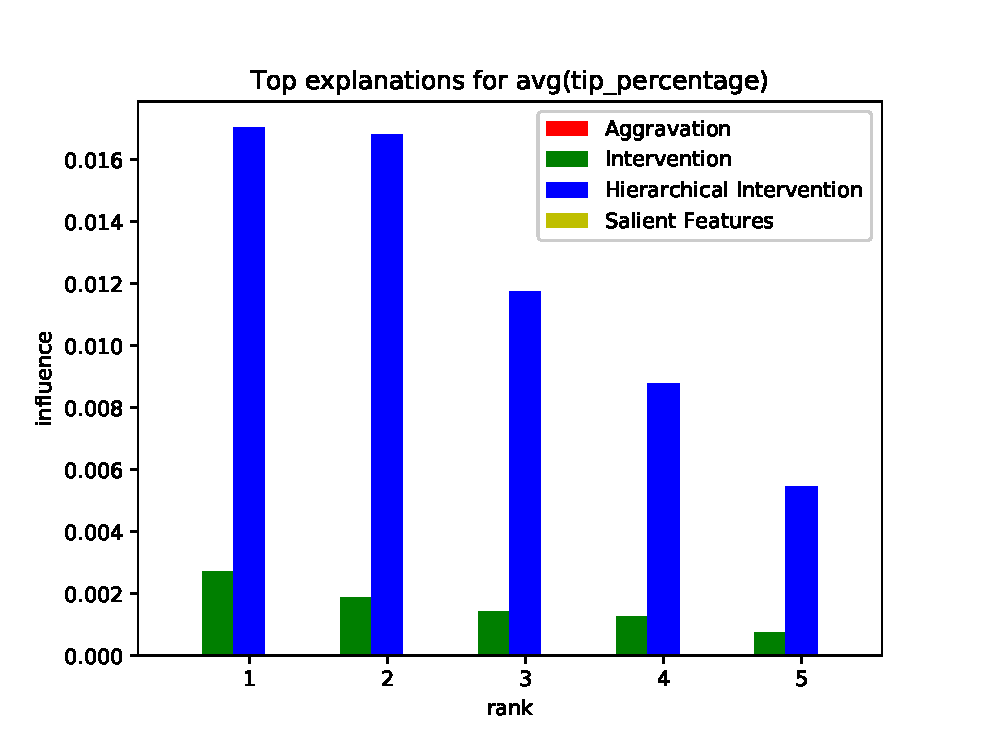
\includegraphics[width=\columnwidth]{Top_explanations_for_avg_tip_percentage_influence}
\caption{Influence for Spatial explanation for average tip percentage(Lower is better)}
\label{fig:influence_comparison}
\end{figure}

Fig.~\ref{fig:influence_comparison} shows the comparison between the influence for different approaches. Salient features and Aggravation have a very low influence compared to Intervention and hierarchical intervention. This is because the explanations provided by those approaches cover a very small portion of the entire dataset. This makes removing the associated data have a negligible impact on the entire data.

\section{K-Folds cross validation}
In order to qualitatively assess the solutions, we use K-Folds cross validation\citep{refaeilzadeh2009cross}. Since we do not have ground truth for our explanations, we have to make a compromise in terms of estimating how good our solution is. Our assumption here is that in general a good explanation would stand out on unseen data i.e. given a good explanation on part of the data, it would give similar results on unseen parts of the data. We split the data into $k$ parts. One of the parts is used to find the explanation(the training data). The rest of the data is the test data. We also calculate an explanation for the test data. The relative distance between the explanation index of the test data and the explanation index of the explanation provided by the training data when applied to the test data is used as a measure of evaluation. 
There is a reason for applying the explanation provided by the training data to the test data. The observation can be anything. The size of the training and test data is different depending on $k$. The observation can depend on the size of the data. This adds a bias when the explanation index for the training data is compared with the explanation index of the test data. Thus, we must apply the explanation provided by the training data on the test data and compare it with explanation when we apply the approach on the test data.

\begin{figure}[h]
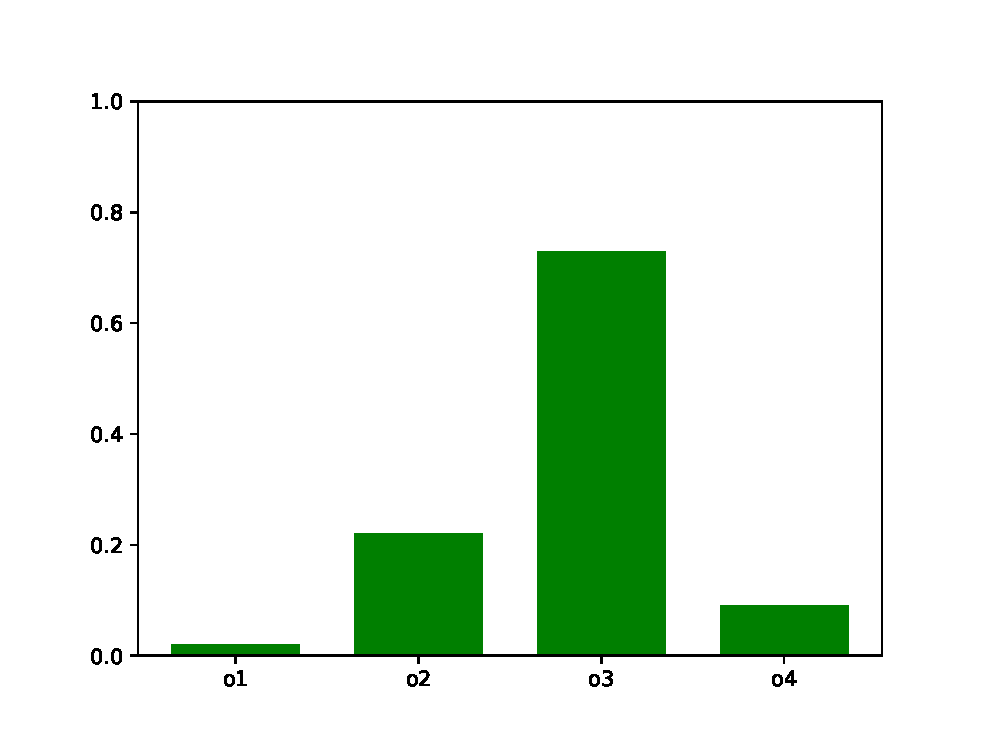
\includegraphics[width=\columnwidth]{kfoldsevaluation}
\caption{The result for k-folds evaluation shows good results when the approach is used in favor of influence(lower is better)}
\label{fig:kfolds}
\end{figure}

We performed evaluation on the first 5 months of data from the NYC yellow cab dataset from 2016. The data spanned ~ 50 million trips. The $k$ for our evaluation was $5$. Each month represented a partition for k-folds evaluation. According to our analysis, we found that the approach works very well with low values of alpha. Fig.~\ref{fig:kfolds} shows some of the results of our evaluation for a number of observations. The lower the value of the relative distance the better the results.

\section{Precision and Recall}
\begin{wrapfigure}{r}{0.5\textwidth}
  \begin{center}
    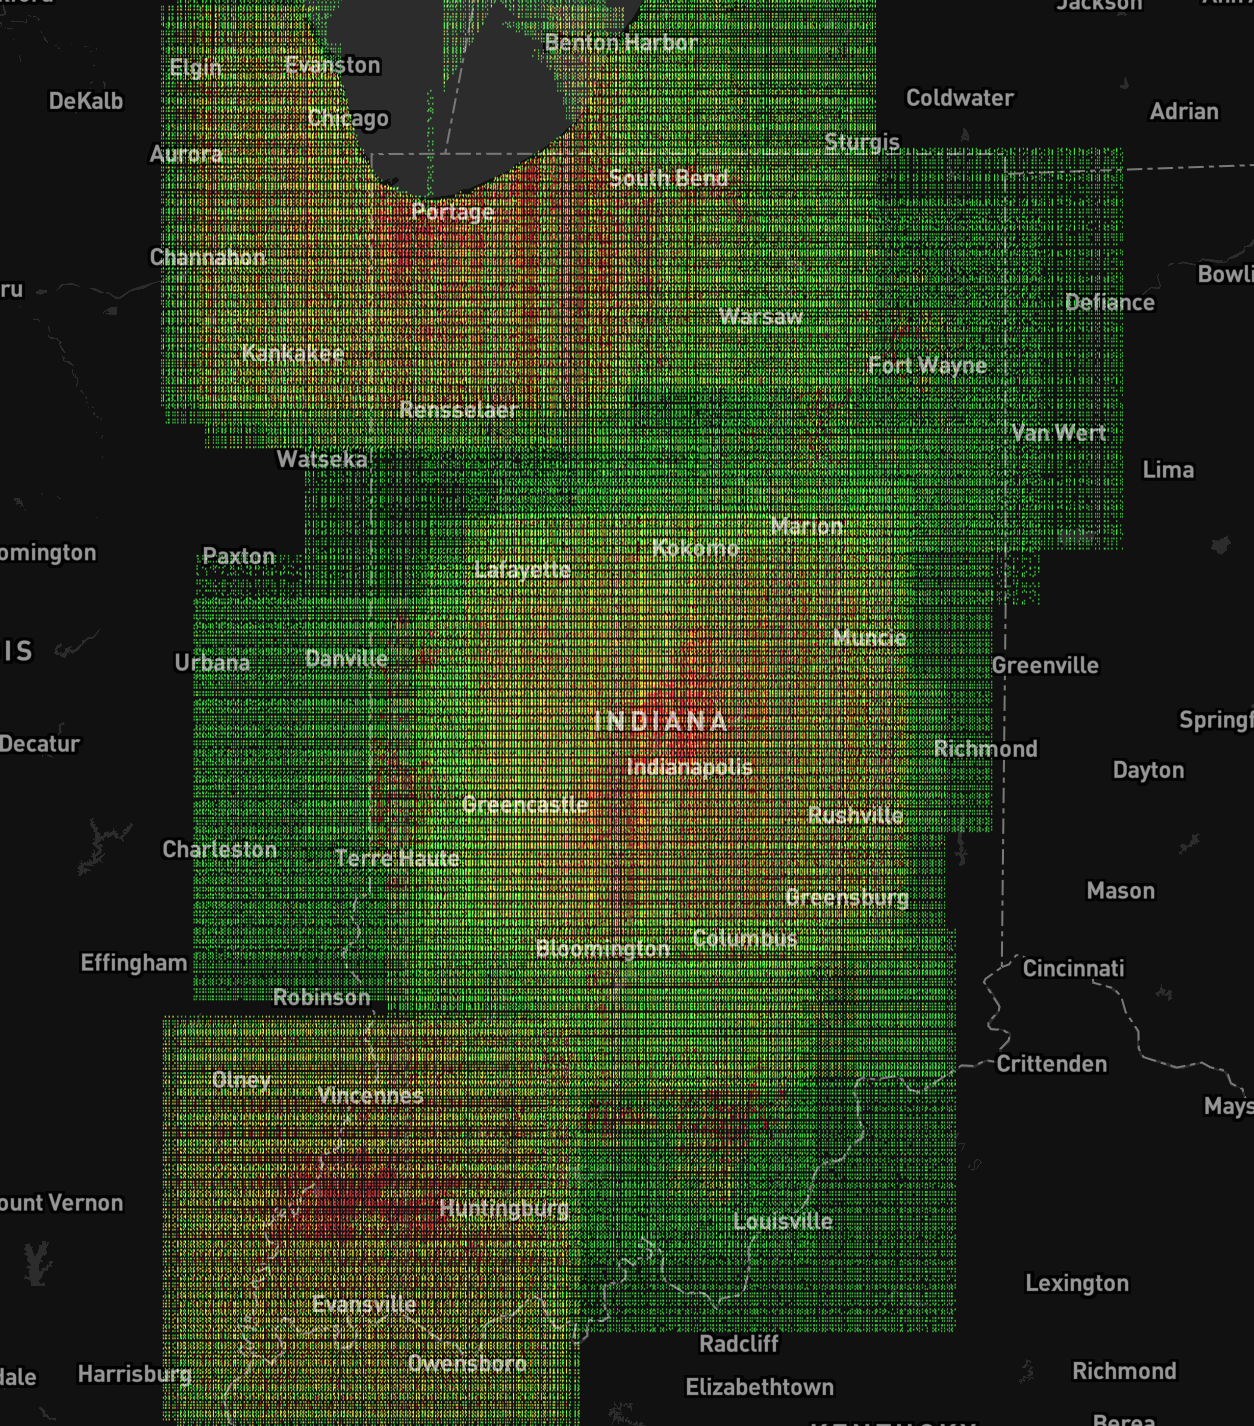
\includegraphics[width=0.48\textwidth]{outbreakheatmap.png}
  \end{center}
  \caption{A heatmap showing sythesized data}
  \label{fig:synthesized_data}
\end{wrapfigure}
% \begin{figure}[h]
% 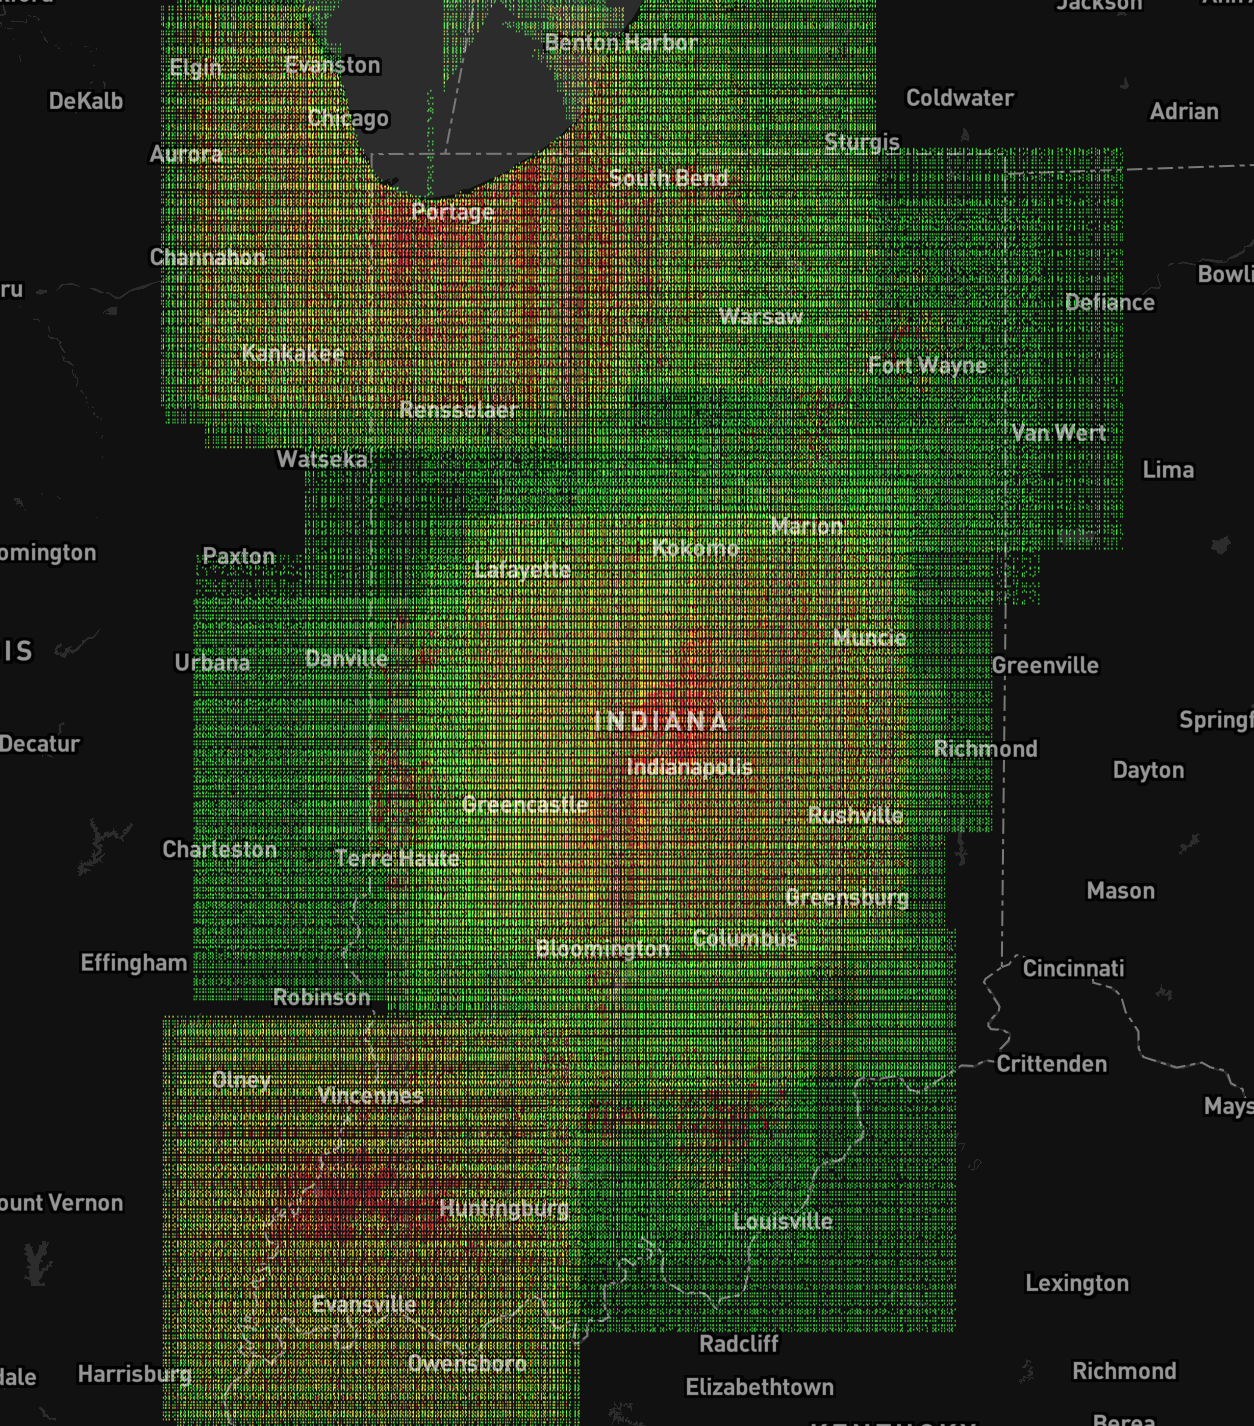
\includegraphics[width=\columnwidth]{outbreakheatmap.png}
% \caption{A heatmap showing sythesized data}
% \label{fig:synthesized_data}
% \end{figure}


Since it is very difficult to find datasets with ground truth we used synthetic datasets to evaluate our solution\citep{maciejewski2009generating}. The synthetic dataset is fabricated using real data from Indiana Public Health Emergency Surveillance System. This data contains information about Patients in Indiana and their health issues over time and location. We can calculate precision and recall using this data\citep{powers2011evaluation}. The data is synthesized in such a way that it shows similar patterns to the actual data. Synthetic data related to outbreaks of certain diseases is synthesized into this data. In order to evaluate our system, we used the temporal component of the outbreak and the type of disease as our observation. To be specific, the synthetic data consisted of an outbreak of Gastrointestinal infection in July. Our observation was the ratio of the number of gastrointestinal infection incidents between June and July when there's an infection against the number of gastrointestinal infection incidents between June and July in synthesized data where there wasn't an outbreak. Precision and Recall was calculated by comparing the areas of the top ten explanations related to the ground truth with the approximate area covered by the outbreak data. We cannot use the individual points to calculate precision and recall because there is a lot of data unrelated to the outbreak which occurs in proximity. To put things into context, each instance of the synthesized data contains ~2 million records. The data related to the outbreak consists of a few dozen records. Fig.~\ref{fig:synthesized_data} shows a heatmap of all the points in the synthesized data. The outbreak for this particular instance only affects a small part of Indiana to the North West just below the river. Fig.~\ref{fig:precisionrecall} shows the points representing the outbreak as well as some of the top polygons returned using Hierarchical Intervention. 

\begin{figure}[h]
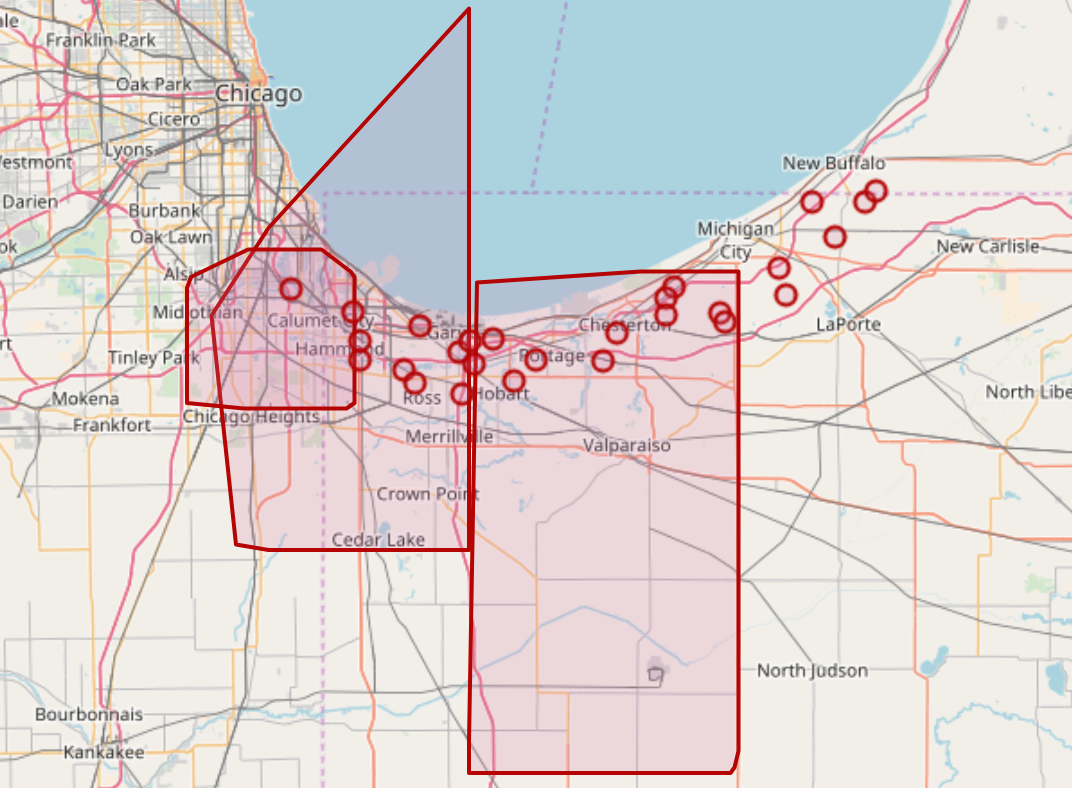
\includegraphics[width=\columnwidth]{precisionrecall.png}
\caption{Synthetic Outbreak data. The circles show the ground truth while the polygons show the relevant explanations produced by our system}
\label{fig:precisionrecall}
\end{figure}

Let $E$ be the area represented by our polygons. Let $O$ be the area represented by the Outbreak points. Then,
$$Precision = \frac{E \cap O}{E} = 0.31$$

For calculating recall, we can use the actual outbreak points since it doesn't require false positives.
$$Recall = \frac{true\_positives}{false\_negatives} = 0.74$$




\subsection{Comparison}
We compared the precision and recall for Hierarchical Intervention with Aggravation and Intervention. 
\\
\textbf{Aggravation}. We used the same observation for aggravation that we did for Hierarchical Intervention. From the top ten explanations, only one of the explanation was able to predict one of the 27 correct tuples in the ground truth.
$$Precision = 0.01$$
$$Recall = 0.04$$


\textbf{Intervention}. Finally Intervention was used to find an explanation. Since there was only one hospital in the area of outbreak, Intervention was able to provide that hospital as a relevant predicate in an explanation. This resulted in all the ground truth points being included in the explanation! However, since there are a large number of tuples related to this predicate, it resulted in a low precision.

$$Precision = 0.0003$$
$$Recall = 1$$


% \begin{wrapfigure}{r}{0.5\textwidth}
%   \begin{center}
%     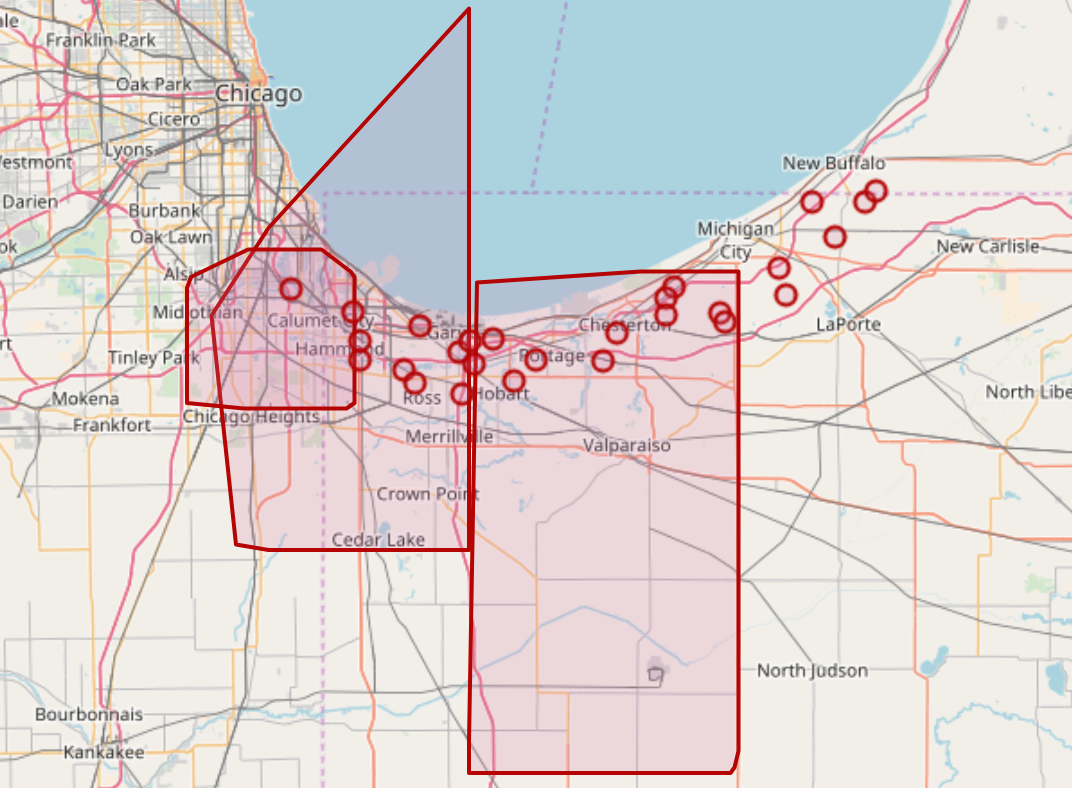
\includegraphics[width=0.48\textwidth]{precisionrecall.png}
%   \end{center}
%   \caption{Synthetic Outbreak data. The circles show the ground truth while the polygons show the relevant explanations produced by our system}
% \label{fig:spatial_spatial_vertical}
% \end{wrapfigure}



% \textbf{Influence and Intensity for Hierarchical Intervention}
% \begin{figure}[H]
% 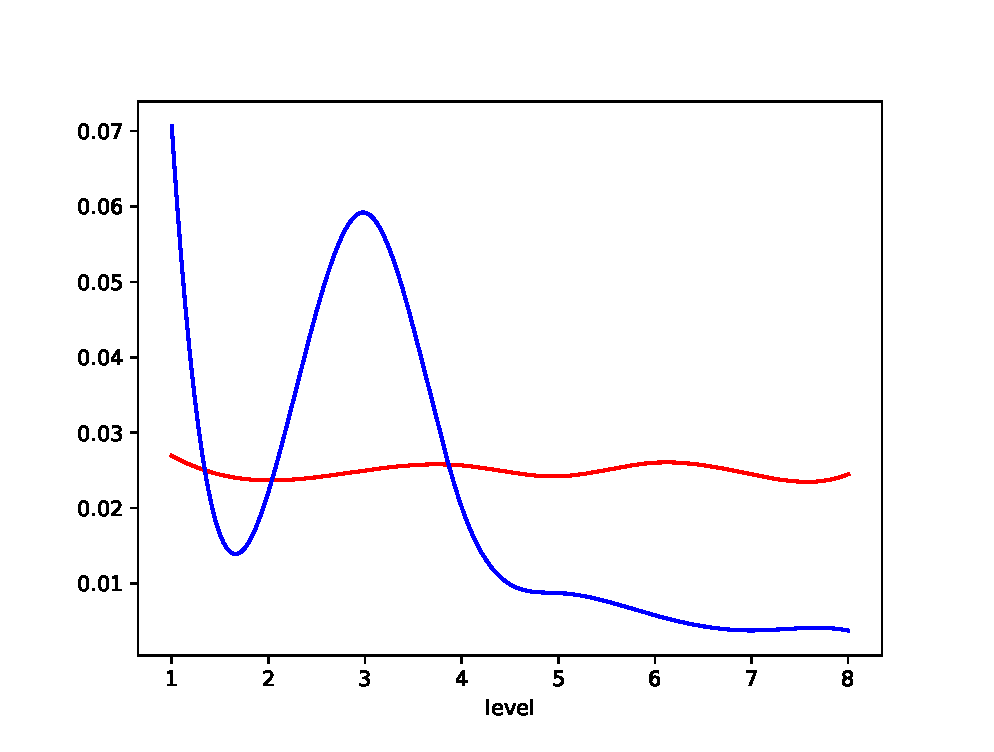
\includegraphics[width=\columnwidth]{heiint_tip_percentage}
% \caption{Comparison of Influence and Intensity against level of hierarchy with average tip percentage as observation}
% \label{fig:hieint_tip_percentage}
% \end{figure}




% \begin{figure}[H]
% 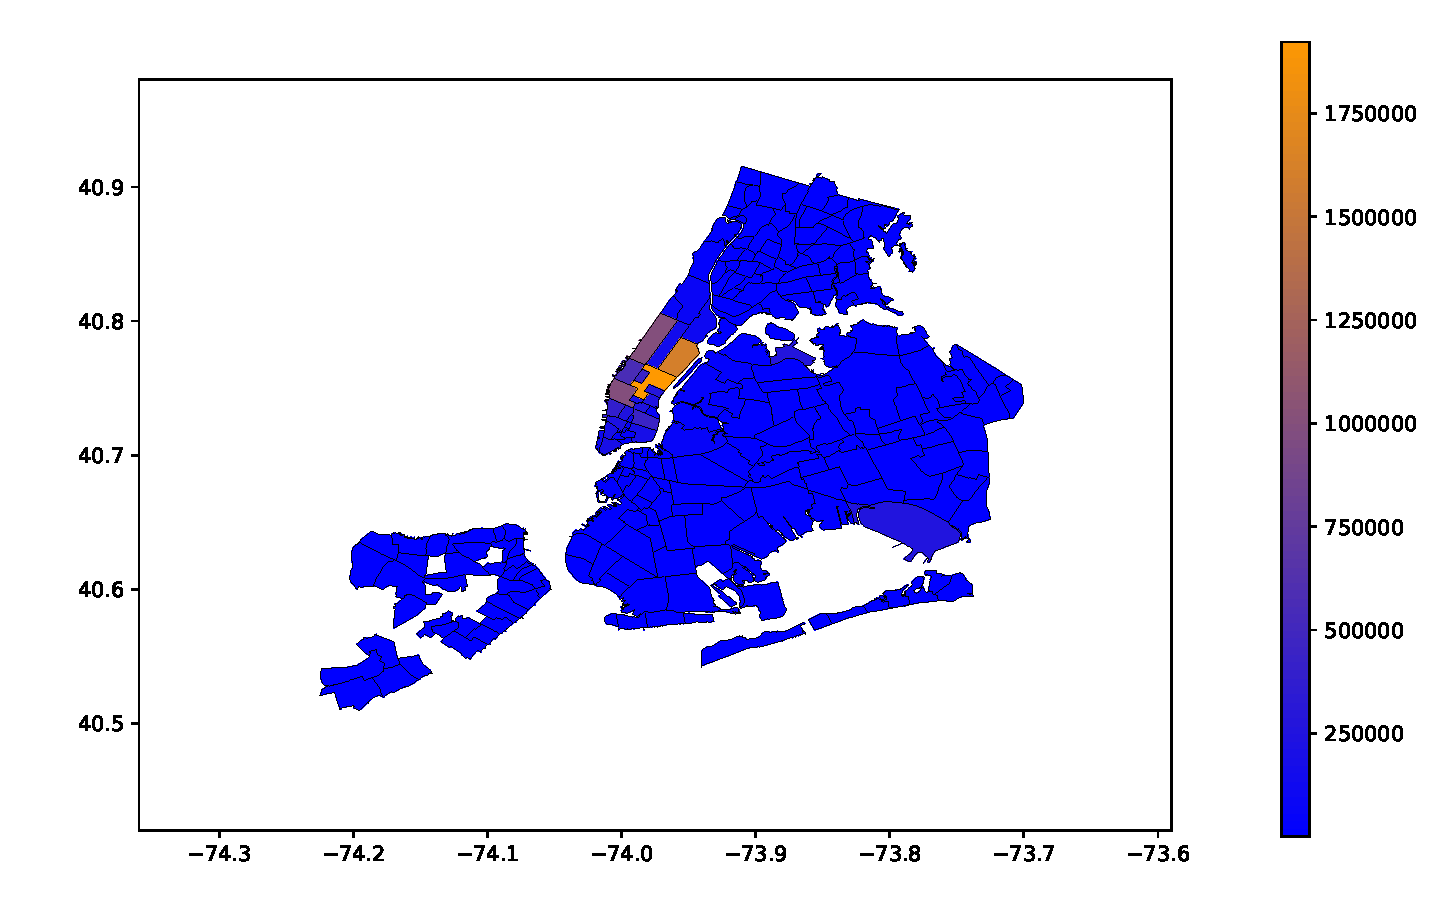
\includegraphics[width=\columnwidth]{count_initial}
% \caption{The number of trips for each zone by pickup zone}
% \label{fig:count_initial}
% \end{figure}

% \begin{figure}[H]
% 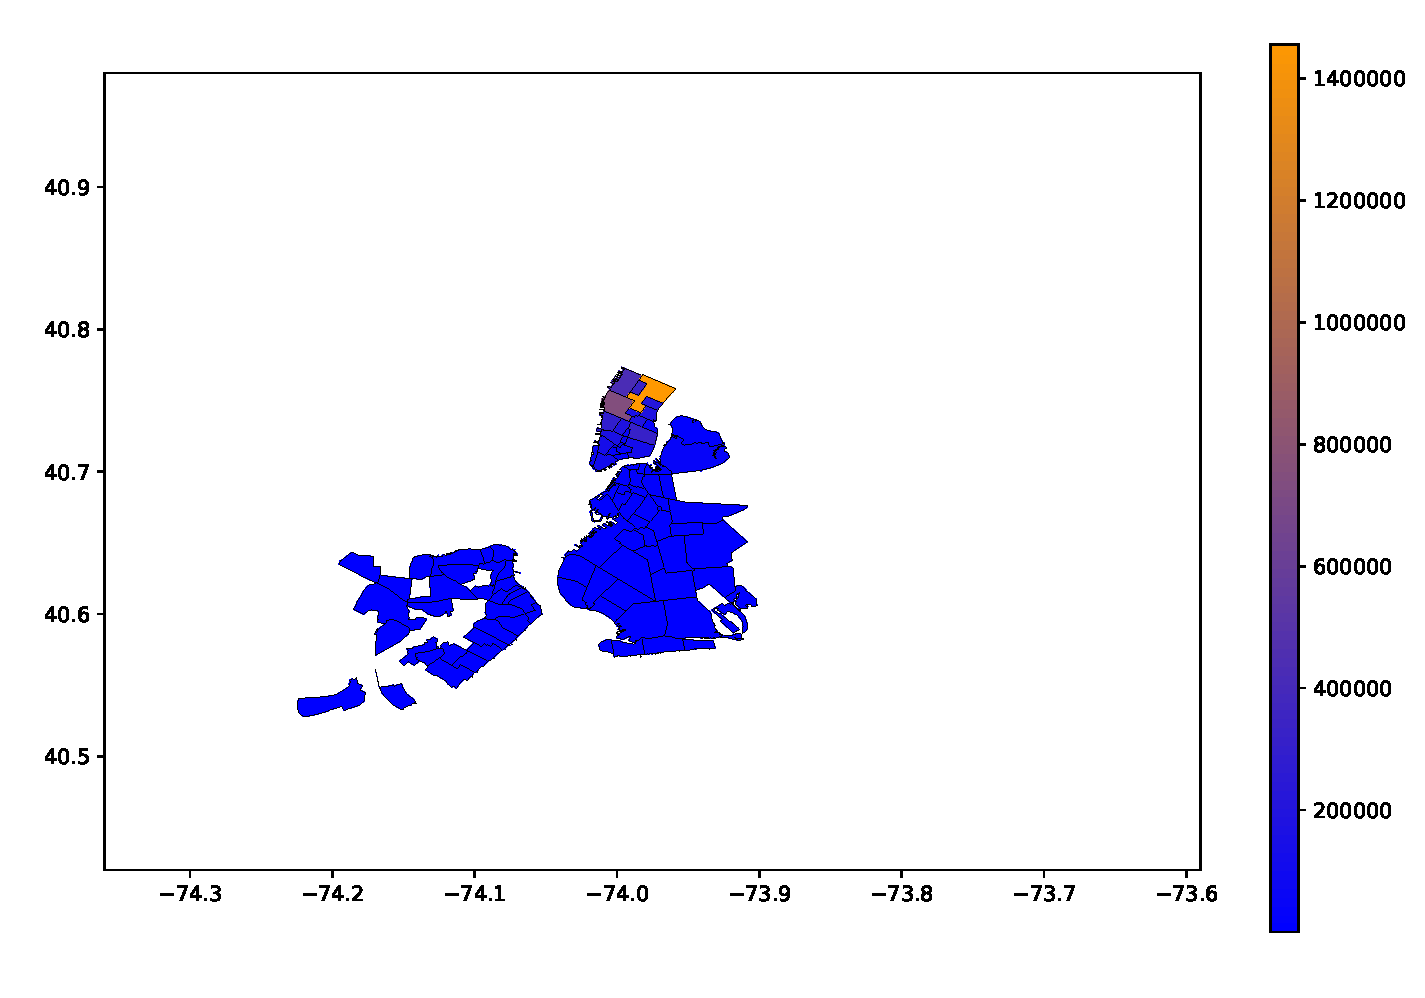
\includegraphics[width=\columnwidth]{top_level_2}
% \caption{Number of rows that represent the top explanation for average tip percentage at level 2}
% \label{fig:top_level_2}
% \end{figure}

% \begin{figure}[H]
% 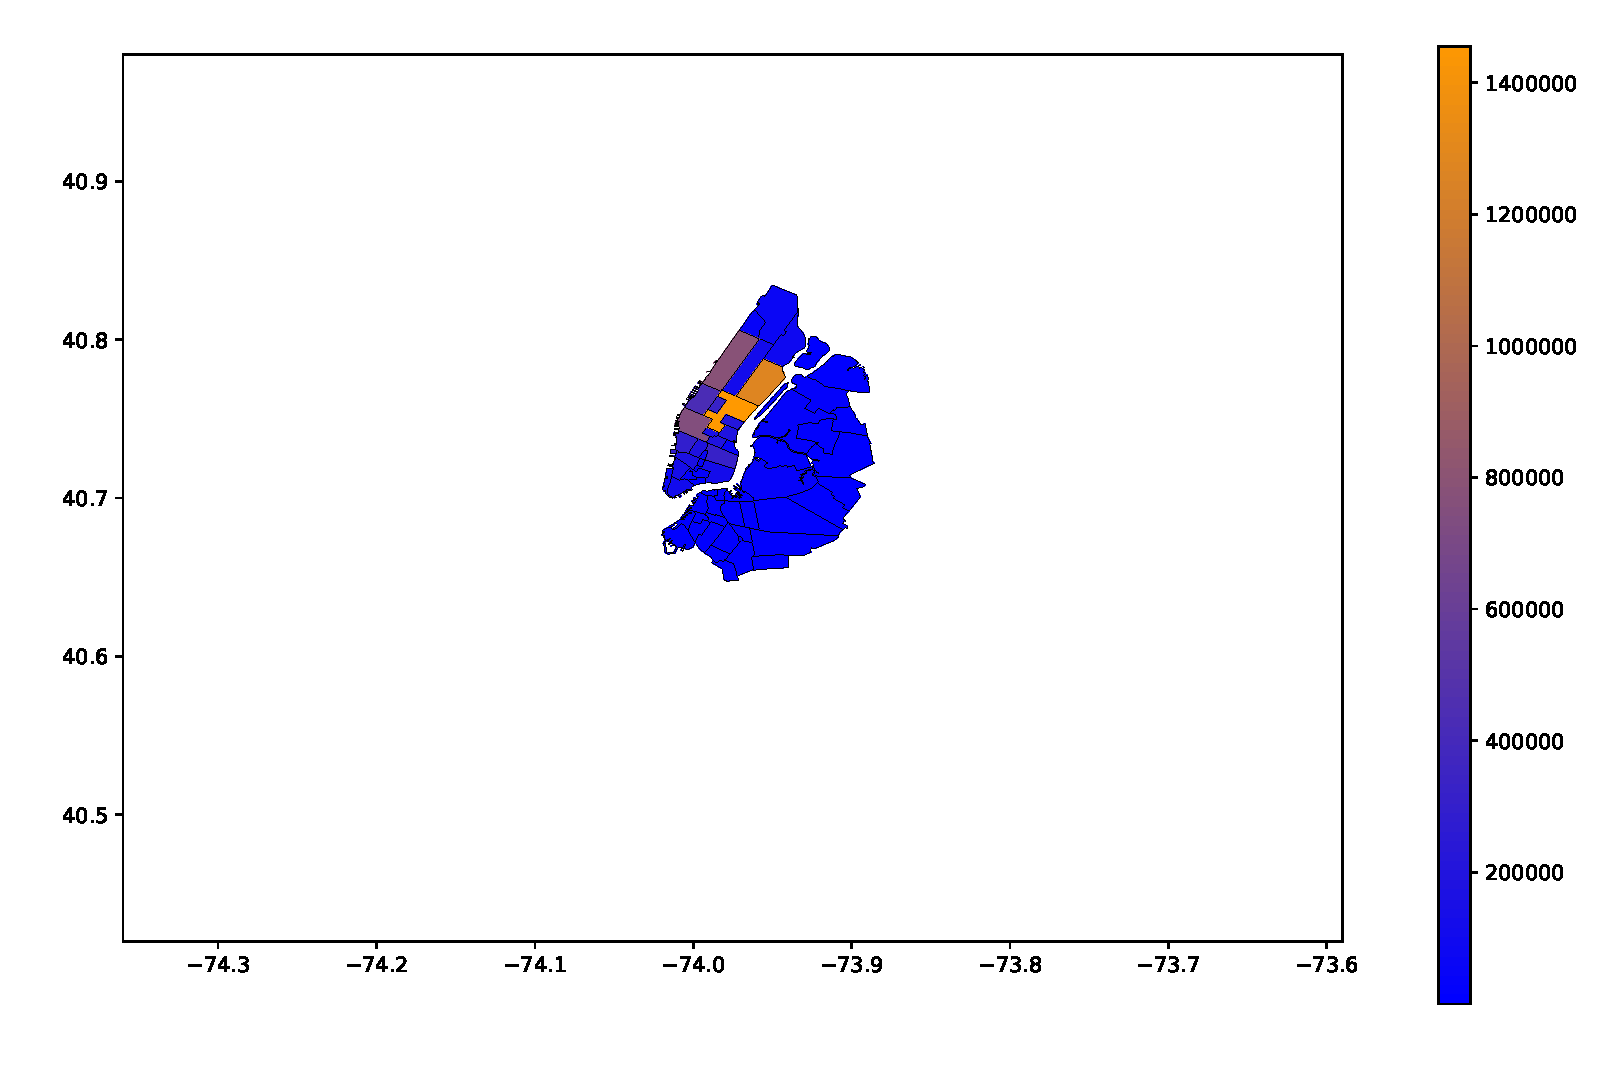
\includegraphics[width=\columnwidth]{top_level_3}
% \caption{Number of rows that represent the top explanation for average tip percentage at level 3}
% \label{fig:top_level_3}
% \end{figure}

% \begin{figure}[H]
% 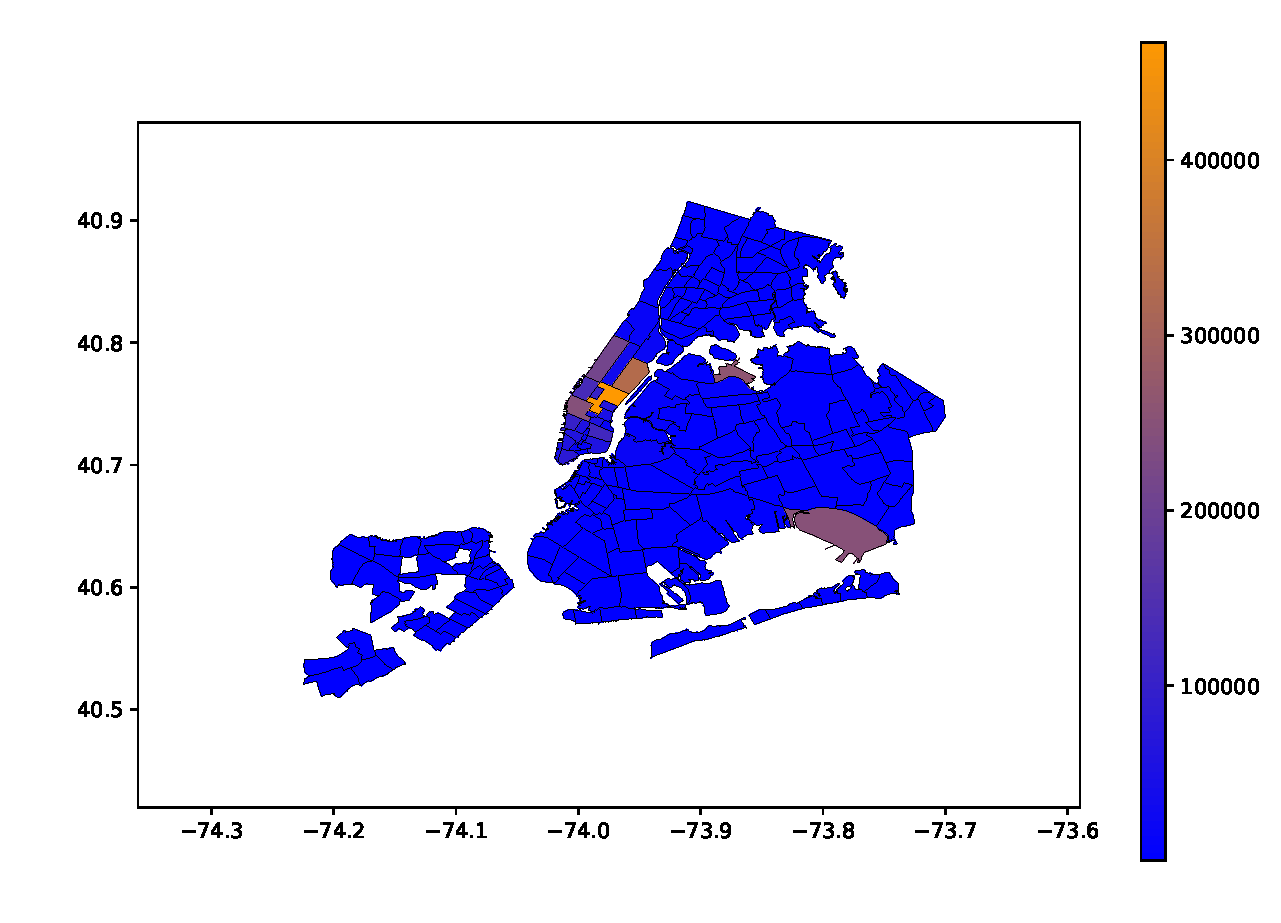
\includegraphics[width=\columnwidth]{level_3_removed}
% \caption{The cartogram for the data when we remove he level 3 explanation}
% \label{fig:level_3_removed}
% \end{figure}


\section{Speed and Scalability}
\label{sec:speed}
The speed of each approach is simply the time taken to calculate the explanations. The time varies depending on the size of the data. For performance evaluation, we used the NYC TLC data for 2016. The data is divided into months. As we increase the number of months to be processed, the time taken for each approach increases almost linearly for aggravation, intervention and hierarchical intervention. For salient features, the time increases slightly exponentially. The results of our evaluation are displayed in Fig.~\ref{fig:performance}
% The speed of each approach is simply the time taken to calculate the explanations. Since all the approaches are implemented on top of distributed systems, the time varies depending on the number of nodes used. We experimented with calculating explanations for 1,3, and 5 nodes in a distributed environment. For the cluster we used Google Compute Engine nodes(1 vCPU, 3.5GB RAM). All the nodes in our cluster had the same specifications. The Aggravation, Intervention and Spatial Intervention were tested on Apache Spark running on YARN while the Salient Features were generated with the Data Polygamy Framework running on YARN. 
\begin{figure}[h]
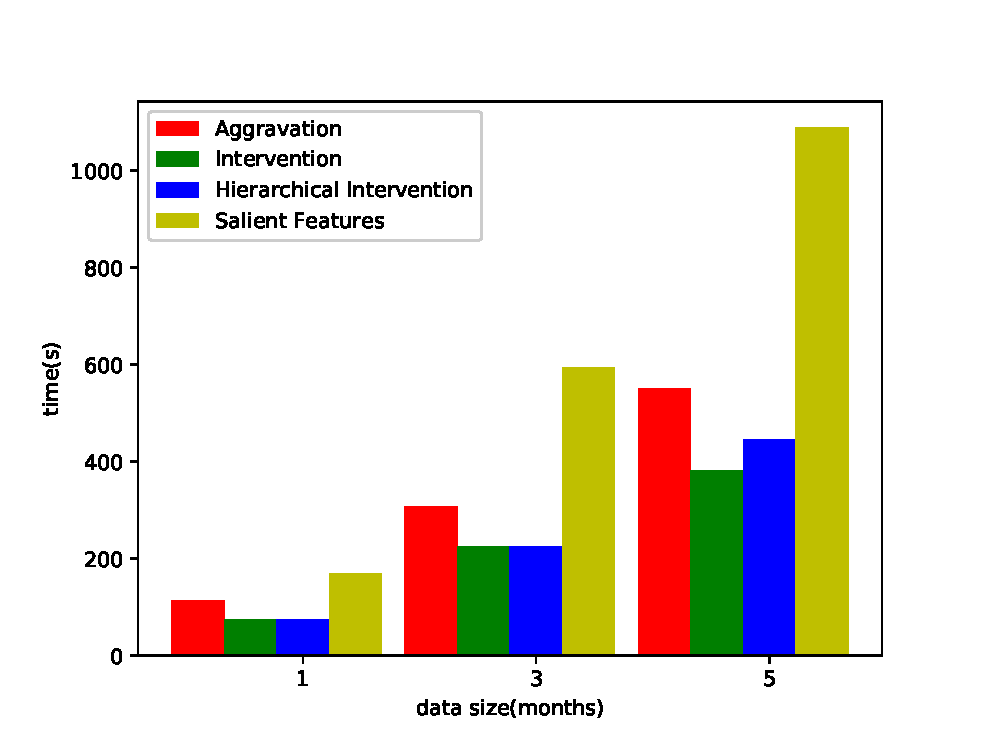
\includegraphics[width=\columnwidth]{performance}
\caption{Time taken by each approach as we increase the size of data}
\label{fig:performance}
\end{figure}



% \begin{figure}[H]
% 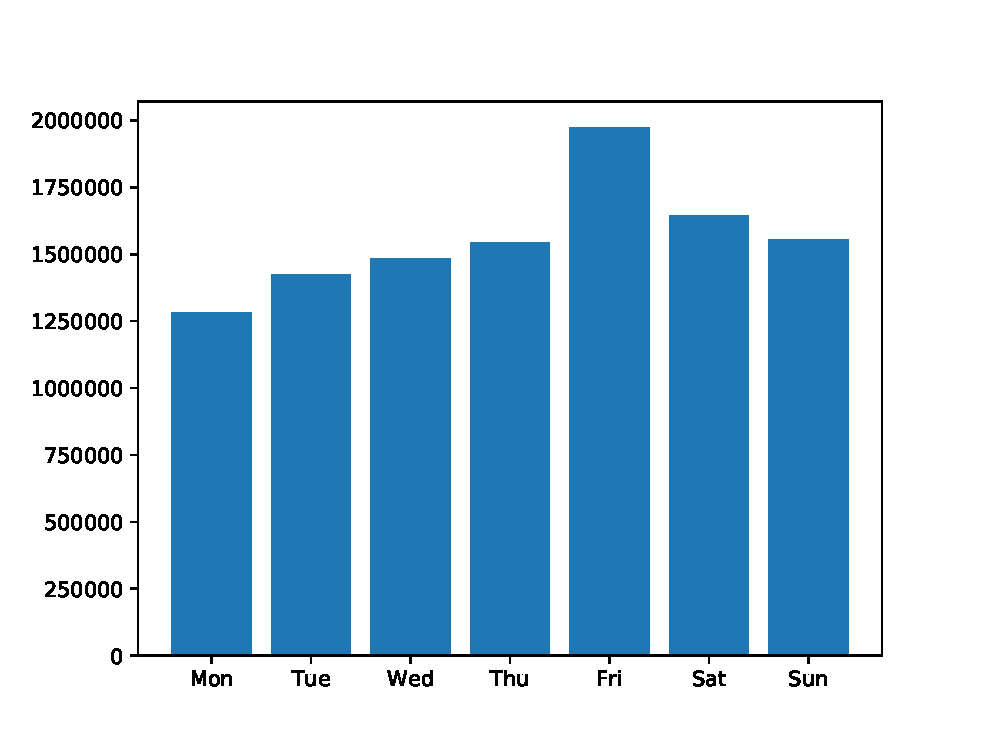
\includegraphics[width=\columnwidth]{day_comparison}
% \caption{Number of trips against trip day}
% \label{fig:day_comparison}
% \end{figure}